%% Sampling an amplitude
%
% An amplitude of a matrix product state: psi(s_1, ..., s_5), every physical
% index closed by a basis vector.
%
% This is what sampling evaluates. With the center on the first site and every
% tensor to its right isometric, the marginal of s_1 needs only C -- the rest
% of the chain contracts to the identity -- so s_1 is drawn first, fixed, and
% the center moves on; each later s_i is conditioned on the ones before it in
% the same way, and the sample costs one sweep.
%
% The basis vectors are a layer of their own, small circles, each closing the
% index above it.
\documentclass[border=4pt]{standalone}
\usepackage{amsmath,amssymb}
\usepackage{tikz-tensors}
\input{notation}
\begin{document}
\begin{tikzpicture}
  \tnstack{S}{5}{ket, basis}
  \tnlayer{S}{ket}{center/$C$, 4*canr/$B$}
  \tnlayer{S}{basis}{basis/$s_1$, basis/$s_2$, basis/$s_3$, basis/$s_4$,
                     basis/$s_5$}
  \tnconnect[along=gauge]{S}
\end{tikzpicture}
\end{document}
